
\subsection{LM-band imaging}
\label{sec:recipes_img_lm}

\subsubsection{LM-band imaging flatfield}
\label{sssec:lm_img_flatfield}

The purpose of the flat-field calibration is to determine
pixel-to-pixel gain variations and large scale illumination variations
(due to inhomogeneities of optical elements in the telescope or
instrument). Calibration frames are obtained either during day time
using the black-body lamp of the \ac{WCU} (internal flats) or by taken
images of the twilight sky (twilight flats). Advantages and
disadvantages of the two types of flat are discussed in
\cite{METIS-calibration_plan}. Since the operational concept for
twilight flats needs to be refined during commissioning at the
telescope, the current recipe design is primarily valid for internal
flats.

This recipe creates a master flat for the HAWAII2RG detector (LM-band
imaging) from lamp or sky images matched by various setup parameters
as detailed below.  A set of internal flats includes a number of
exposures with \CODE{LAMP OFF}, which will be used for dark
subtraction. For twilight flats a master dark will be subtracted. The
master flat is obtained by the slope of a linear fit of the pixel
values against the illumination level of the exposures.

The quality control parameters give various statistics for each input
frame (mean, standard deviation, etc.), the standard deviation of the
normalised master flat and the number of bad pixels identified by the
recipe. If a bad-pixel map is provided on input, it is updated,
otherwise a new one is created.

\begin{recipedef}
  Name:                & \REC{metis_lm_img_flat}                                    \\
  Purpose:             & Create master flat field for the LM-band imaging detector. \\
  Requirements:        & \REQ{METIS-6096}                                           \\
  Type:                & Calibration                                                \\
  Templates:           & \TPL{METIS_img_lm_cal_LampFlat}                            \\
                       & \TPL{METIS_all_cal_TwilightFlat}                           \\
  Input data:          & Flat field images taken with lamp or sky.                  \\
                       & Master dark (for twilight flats)                           \\
                       & Bad pixel map                                              \\
  Matched keywords:    & Detector ID                                                \\
                       & Filter ID                                                  \\
                       & ADC ID                                                     \\
                       & possibly others (e.g.\ coronagraphic mask, \TBD)           \\
  Recipe parameters:   & Combination method (\texttt{mean}, \texttt{median},
                         \texttt{sigclip}, \dots)                                \\
                       & Parameters for combination methods                         \\
                       & Threshold for bad-pixel identification                     \\
  Algorithm:           & For internal flats: combine \CODE{LAMP OFF} exposures to dark. \\
                       & Subtract internal dark or master dark from flat exposures. \\
                       & Fit slope of pixel values against illumination level.      \\
                       & Add pixels with significant deviations to bad pixel map.   \\
  Output data:         & \PROD{MASTER_IMG_FLAT_2RG}                                 \\
                       & \PROD{BADPIX_MAP_2RG}                                      \\
  Expected accuracies: & \TBD                                                       \\
  QC1 parameters:      & \QC{QC LM MASTERFLAT RMS}                                  \\
                       & \QC{QC LM FLAT NBADPIX}                                    \\
                       & \QC{QC LM FLAT MEAN ##}                                    \\
                       & \QC{QC LM FLAT RMS ##}                                     \\
  hdrl function        & \CODE{hdrl_bpm_fit_compute}                                \\
                       & \CODE{hdrl_imagelist_collapse}                             \\
                       & \CODE{hdrl_imagelist_sub_image}                            \\
\end{recipedef}

\begin{figure}[hb]
  \centering
  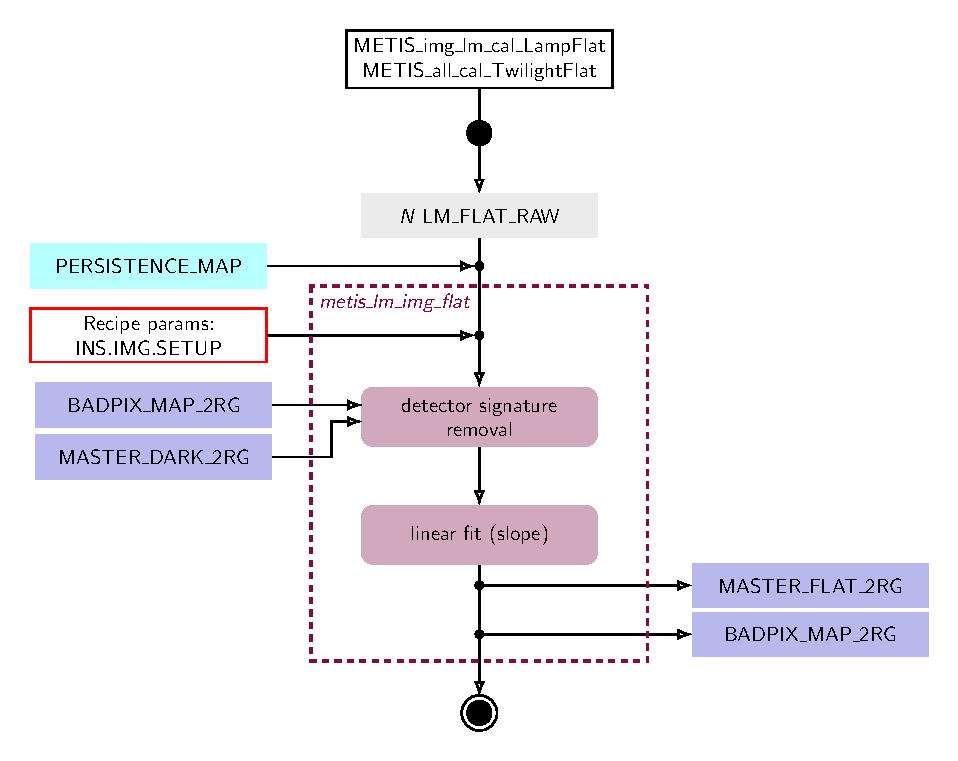
\includegraphics[width=0.6\textwidth]{metis_lm_img_flat}
  \caption[Recipe: \REC{metis_lm_img_flat}]{\REC{metis_lm_img_flat} --
    creation of \CODE{IMG_LM} master flatfield.\\ \TODO{Include averaging of
      frames at same illumination}}
  \label{fig:metis_lm_img_flat}
\end{figure}


\clearpage
\subsubsection{LM-band imaging basic reduction}
\label{sssec:lm_img_basic}

\textbf{New recipe -- this may be too basic and could be joined with
  the background subtraction.}

This recipe performs the basic reduction of raw exposures from the
LM-band imager, i.e.\ dark subtraction and flat fielding. It is used
for both standard and science exposures.

Basic statistics of the images can be used to screen for saturation.

\TODO{This recipe should analyse the masked detector regions for
  channel offset correction and crosstalk (see \cite{matisse_minutes}).}

\begin{recipedef}
  Recipe name:      & \REC{metis_lm_img_basic_reduce}   \\
  Purpose:          & apply basic reduction of images   \\
  Type:             & Calibration, Science              \\
  Templates:        & \TPL{METIS_img_lm_cal_standard}  \\
                    & \TPL{METIS_img_lm_*_obs_*}       \\
  Input data:       & Dithered images (standard, science) \\
                    & Blank sky images (if available)   \\
                    & Master dark                       \\
                    & Master flat                       \\
  Matched keywords: & DIT (for dark)                    \\
                    & Filter ID (for flat)              \\
  Algorithm:        & Subtract dark, divide by flat     \\
                    & Analyse and remove masked regions (\TBD) \\
  Output data:      & \PROD{LM_SCI_BASIC_REDUCED}       \\
                    & \PROD{LM_STD_BASIC_REDUCED}       \\
  QC1 parameters:   & \QC{QC LM IMG MEDIAN}             \\
                    & \QC{QC LM IMG PEAK}               \\
  hdrl functions:   & \CODE{hdrl_imagelist_sub_image}   \\
                    & \CODE{hdrl_imagelist_div_image}   \\
\end{recipedef}

\begin{figure}[hb]
  \centering
  % 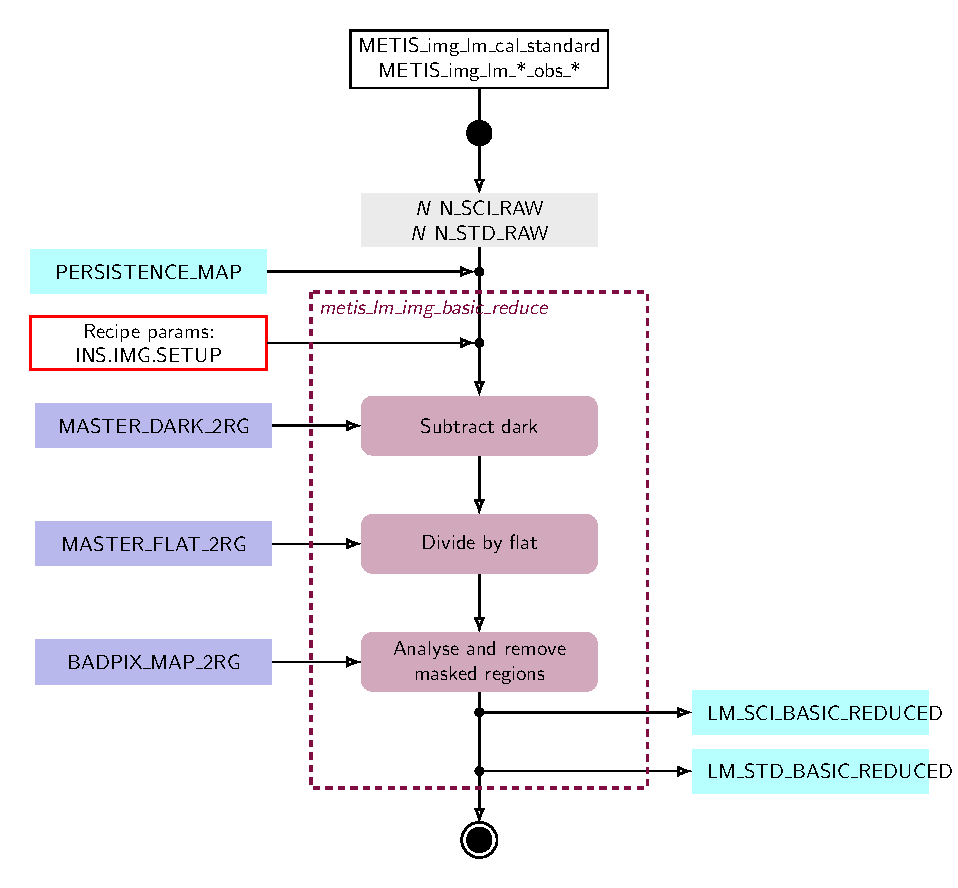
\includegraphics[width=0.6\textwidth]{metis_lm_img_basic_reduce}
  \resizebox{0.6\textwidth}{0.1\textwidth}{\TODO{\fbox{Figure to be done}}}
  \caption[Recipe: \REC{metis_lm_img_basic_reduce}]{\REC{metis_lm_img_basic_reduce} --
    basic reduction of \CODE{IMG_LM} data.}
  \label{fig:metis_lm_img_basic_reduce}
\end{figure}


\clearpage
\subsubsection{LM-band imaging background subtraction}
\label{sssec:lm_img_background}

This recipe estimates and subtracts the background from LM-band
imaging data. Thermal background emission from the atmosphere,
telescope and warm parts of the instrument dominate the photon count
in mid-infrared observations. Accurate determination and removal of
background counts is therefore crucial to make MIR data scientifically
usable.

A set of observations will consist of a number of dithered exposures
of the field, where the offsets are achieved using the internal
chopper of METIS or the with the telescope. For extended objects, the
telescope will be used to perform ``out-of-field dithering'', i.e.\
observe nearby blank patches of sky interlaced with the target
observations. Imaging observations are performed in pupil-tracking
mode, hence angular dithering of the field is automatic.

For in-field-dithered exposures, all dithered exposures will be
averaged to obtain the background estimate. In order to only average
the background contribution, an iterative procedure of object
detection and masking will be employed. Averaging will be done using a
robust estimator of the mean (e.g.\ median).

For extended objects, all out-of-field exposures will be averaged
(with object rejection) and subtracted off the in-field exposures.

\TODO{Is this good enough for HCI images or do we need more?}

\begin{recipedef}
  Recipe name:      & \REC{metis_lm_img_background}                             \\
  Purpose:          & estimate and subtract background                          \\
  Type:             & Calibration                                               \\
  Templates:        & \TPL{METIS_img_lm_cal_standard}                           \\
                    & \TPL{METIS_img_lm_*_obs_*}                                \\
  Input data:       & \CODE{LM_SCI_BASIC_REDUCED}                               \\
                    & \CODE{LM_STD_BASIC_REDUCED}                               \\
  Matched keywords: & dither position (\CODE{SKY}? \TBD)                        \\
  Algorithm:        & Average all or \CODE{SKY} exposures with object rejection \\
                    & Subtract background                                       \\
  Output data:      & \PROD{LM_SCI_BKG}                                         \\
                    & \PROD{LM_SCI_BKG_SUBTRACTED}                              \\
                    & \PROD{LM_STD_BKG_SUBTRACTED}                              \\
  QC1 parameters:   & \QC{QC LM IMG BKG MEDIAN}                                 \\
  hdrl functions:   & \CODE{hdrl_imagelist_sub_image}                           \\
                    & \CODE{hdrl_imagelist_div_image}                           \\
\end{recipedef}

\begin{figure}[hb]
  \centering
  % 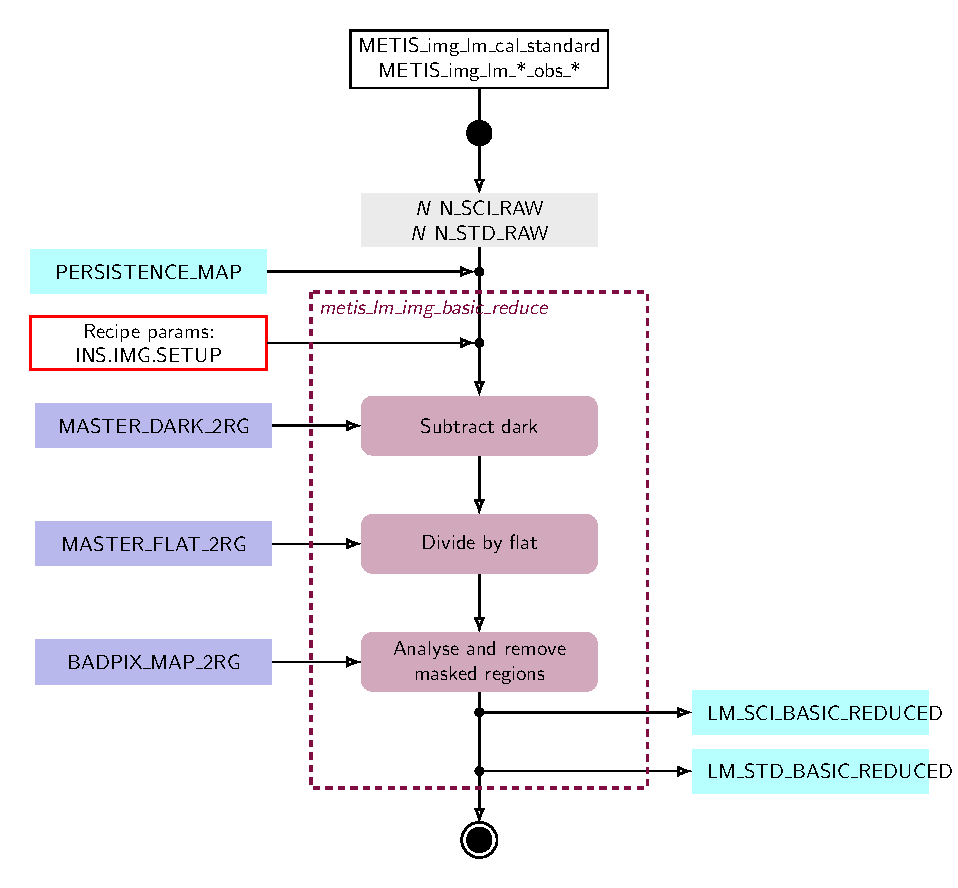
\includegraphics[width=0.6\textwidth]{metis_lm_img_basic_reduce}
  \resizebox{0.6\textwidth}{0.1\textwidth}{\TODO{\fbox{Figure to be done}}}
  \caption[Recipe: \REC{metis_lm_img_basic_reduce}]{\REC{metis_lm_img_background} --
    background estimation and subtraction of dithered \CODE{IMG_LM} data.}
  \label{fig:metis_lm_img_background}
\end{figure}



%%% Local Variables:
%%% TeX-master: "METIS_DRLD"
%%% End:
